\chapter{Optimization}


In \nameref{cannon} in the previous chapter you were asked to find the best launch angle for a human cannonball, meaning the angle that maximizes the distance traveled before landing.  This kind of problem, finding minimums and maximums, is called \emph{optimization}.

In this chapter, we'll solve a similar problem, finding the best launch angle for a baseball.
We'll solve the problem two ways, first running simulations with a range of values and plotting the results, then using a MATLAB function that automates the process, \lstinline{fminsearch}.
\index{baseball}
\index{launch angle}

\section{Optimal Baseball}

In the previous chapter we wrote functions to simulate the flight of a baseball with a known initial velocity.  Now we'll use that code to find the launch angle that maximizes \emph{range}, that is, the distance the ball travels before landing.

\index{optimization}
\index{velocity}
\index{range}

First, we need an event function to stop the simulation when the ball lands.
\begin{code}
function [value, isterminal, direction] = event_landing(t, xx)
    % Event function for ode solver to trigger when vertical position
    % is zero
    value = xx(3);
    isterminal = 1;
    direction = -1;
end
\end{code}

\index{event function}
\index{ODE event}
\index{odeset@\lstinline{odeset}}

This is similar to the event function we saw in Chapter~\ref{events}, except that it uses \lstinline{xx(3)} as the event value, which is the element of the state vector corresponding to the y-position.  This event function stops the simulation when the altitude of the ball is~0 and falling.

Now we can call \lstinline{ode45} like this:
\lstinputlisting[style=mcode, firstline=4, lastline=10]
{../code/chap13/baseball_statespace3.m}


The initial position of the ball is \SI{1}{\meter} above home plate.  The ball's initial velocity is \SI{40}{\meter\per\second} in the $x$-direction and \SI{30}{\meter\per\second} in the $y$-direction.

\index{initial condition}

The maximum duration of the simulation is \SI{10}{\second}, but we expect an event to stop the simulation first.  We can get the final values of the simulation like~this:

\begin{code}
>> tout(end)
ans =
    5.9307
>> Xout(end,:)
ans =
  112.2167   11.9139   -0.0000  -36.2661
\end{code}

The final time is \SI{5.9}{\second}.  The final $x$-position is \SI{112}{\meter}; the final $y$-position is \SI{0}{m}, as expected.



As we saw in Chapter~\ref{projectile}, we can plot the \emph{trajectory} the baseball from launch, on the left, to landing, on the right.  This plot is repeated in Figure~\ref{f:baseball3}

\begin{figure}[h]
\centerline{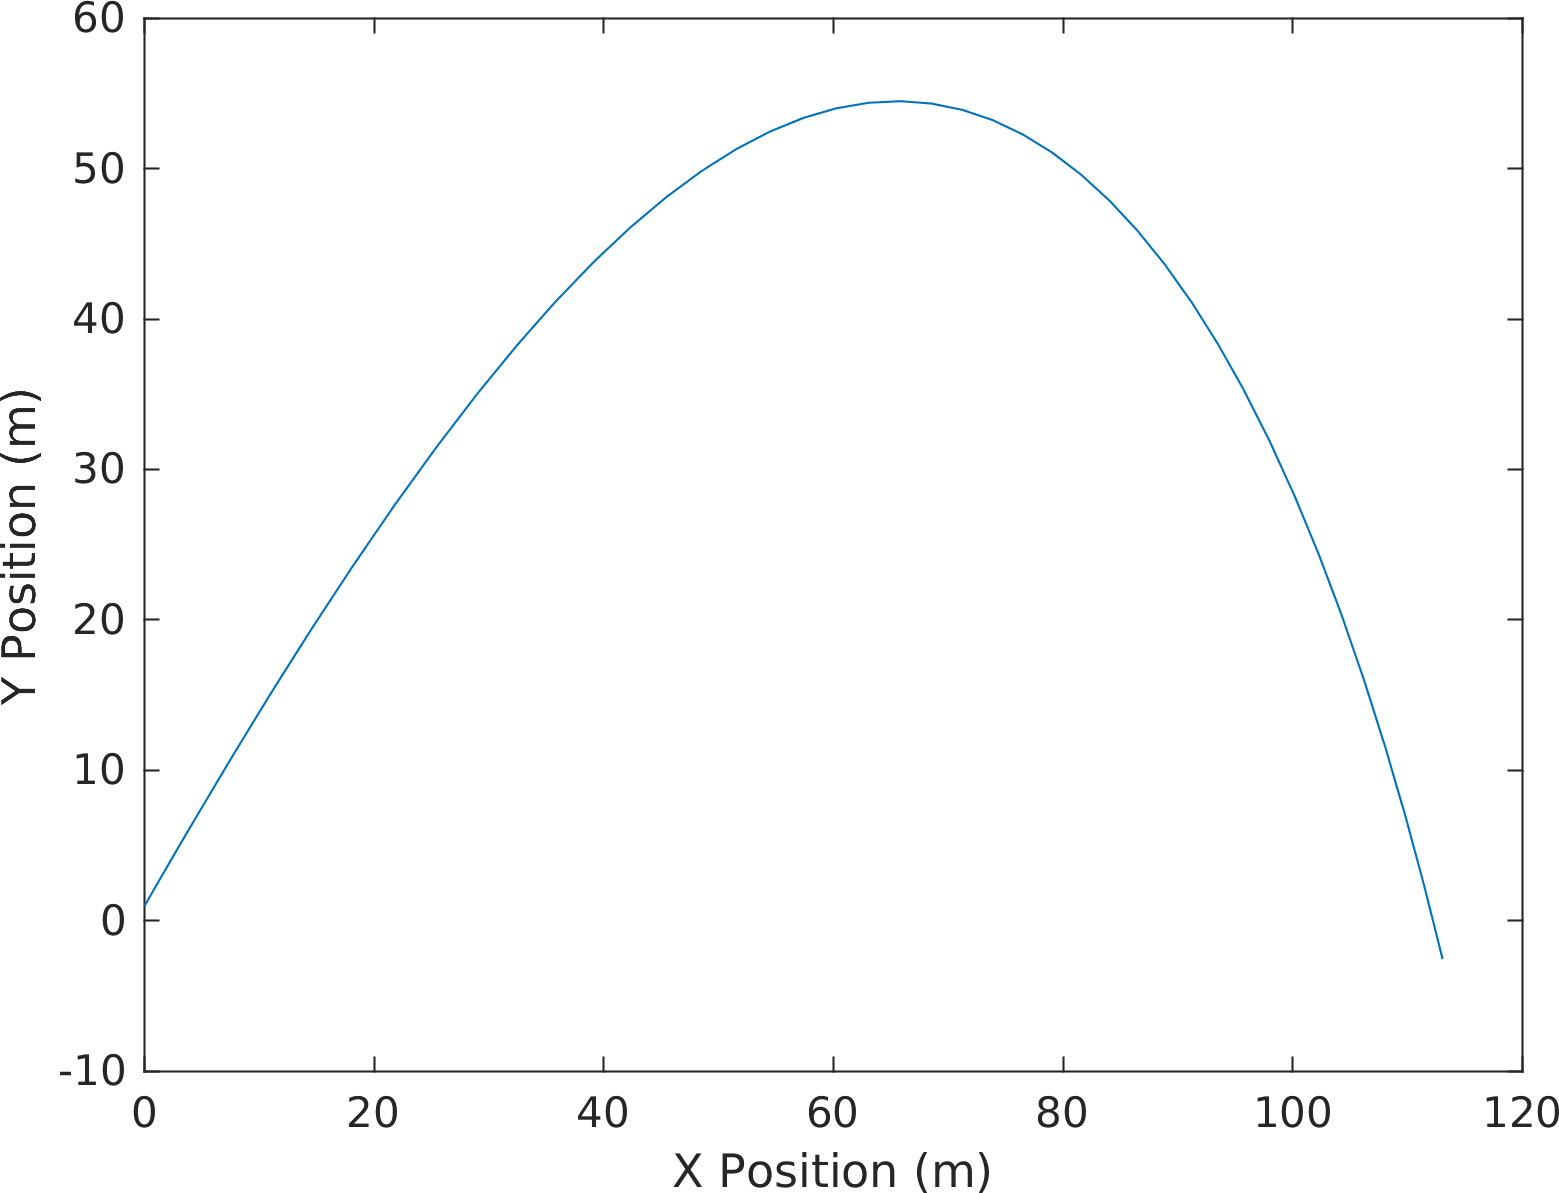
\includegraphics[width=0.7\textwidth]{../code/chap12/baseball2_xy.png}}
\caption{Simulated flight of a baseball plotted as a trajectory}
\label{f:baseball3}
\end{figure}

\index{trajectory}


\section{Exhaustive Search: Range Versus Angle}

Now we'll simulate the trajectory of the baseball with a range of launch angles.  First, we'll take the code we have and wrap it in a function that takes the launch angle as an input variable, runs the simulation, and returns the distance the ball travels (Listing~\ref{lst:baseball_range}).

\index{range}
\index{launch angle}

\begin{lstlisting}[caption={A function that takes the launch angle of a baseball and returns the distance it travels}, label={lst:baseball_range}]
function res = baseball_range(theta)
    P = [0; 1];
    v = 50;
    [vx, vy] = pol2cart(theta, v);

    V = [vx; vy];     % initial velocity in m/s
    W = [P; V];       % initial condition

    tspan = [0 10];
    options = odeset('Events', @event_func);
    [T, M] = ode45(@rate_func, tspan, W, options);

    res = M(end, 1);
end
\end{lstlisting}

The launch angle, \lstinline{theta}, is in radians.  The magnitude of velocity, \lstinline{v}, is always \SI{50}{\meter\per\second}.  We use \lstinline{pol2cart} to convert the angle and magnitude (\emph{polar} coordinates) to Cartesian components, \lstinline{vx} and \lstinline{vy}.

\index{radian}
\index{pol2cart@\lstinline{pol2cart}}
\index{Cartesian coordinates}
\index{polar coordinates}

After running the simulation we extract the final $x$-position and return it as an output variable.

We can run this function for a range of angles like this:

\begin{code}
    thetas = linspace(0, pi/2);
    for i = 1:length(thetas)
        ranges(i) = baseball_range(thetas(i));
    end
\end{code}
And then plot \lstinline{ranges} as a function of \lstinline{thetas}:

\begin{code}
    plot(thetas, ranges)
\end{code}

Figure~\ref{fig:baseball4} shows the result.  As expected, the ball does not travel far if it's hit nearly horizontal or vertical.
The peak is apparently near \SI{0.7}{\radian}.  This is an example of the most basic optimization technique, \emph{exhaustive search}.  In this case, it is computationally feasible to generate (almost) the entire solutions space, the full set of possible launch angles, and then simply select the best one.  

\begin{figure}[h]
\centerline{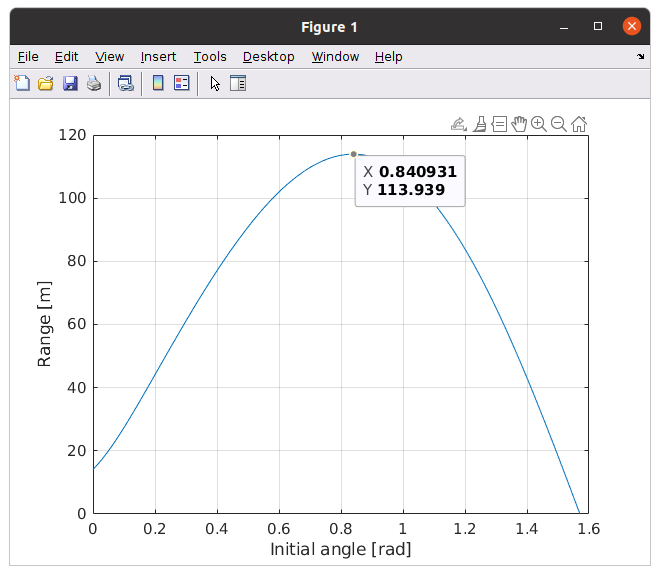
\includegraphics[width=0.7\textwidth]{../code/chap13/range_exhaustive.png}}
\caption{Exhaustive search for maximum range using the \emph{Data tips} graphical tool to choose the near-optimal solution}
\label{fig:baseball4}
\end{figure}


Considering that our model is only approximate, this result might be good enough.  But if we want to find the peak more precisely, we can use \lstinline{fminsearch}.


\section{fminsearch}

The \href{https://www.mathworks.com/help/matlab/ref/fminsearch.html}{\lstinline{fminsearch}} function is similar to \lstinline{fzero}, which we saw in Chapter~\ref{fzero}.  Recall that \lstinline{fzero} takes a function handle and an initial guess, and it returns a root of the function.  The \lstinline{fminsearch} function uses this same interface to implement a nonlinear optimization to search for a value that minimizes the user-supplied function.


If we want to find the maximum of a function, rather than the minimum, we can still use \lstinline{fminsearch} by writing a short function that negates the function we want to maximize.
In the baseball example, the function we want to maximize is \lstinline{baseball_range}; we can wrap it in another function like~this:

\begin{code}
function nrange = negative_range(theta)
% Return -1*range for use with function minimization
nrange = -1.0*baseball_range(theta);
end
\end{code}

And then we call \lstinline{fminsearch} like this:

\begin{code}
    % Inital estimate of solution
    theta0 = 0;
    % Optimization
    [x, fval] = fminsearch(@negative_range, theta0)
\end{code}
which would return
\begin{code}
    x =
    0.8403
fval =
 -113.9392
\end{code}

The optimal launch angle for the baseball is \SI{0.84}{\radian}; launched at that angle, the ball travels almost \SI{114}{\meter}.

If you're curious about how \lstinline{fminsearch} works, see ``\nameref{howfminsearch}'' on page~\pageref{howfminsearch}.

\section{Checking for Logical Errors}

The \lstinline{fminsearch} algorithm often does a great job of finding a local minimum for a wide range of non-linear function, but there are lots of ways that things can go wrong.  This is a common issue with black-box solutions where the process of finding the solution is not clear.   The best way to avoid these logical bugs---where the program is doing exactly what we told it, but still doesn't give the result we intended---is to peer into the black-box. We can do this by setting some of the options available in the \lstinline{fminsearch} interface and looking at more of the outputs.  Here is an example:

\begin{code}
    % Optimization options
    options = optimset('Display','iter', ...
        'PlotFcns', {@optimplotx, @optimplotfval, @optimplotfunccount});
    % Call optimization
    [x, fval, exitflag, output] = fminsearch(@negative_range, theta0, options)
\end{code}

In the snippet above we use the \href{https://www.mathworks.com/help/matlab/ref/optimset.html}{\lstinline{optimset}} function to set parameters to values.  This is a common idiom in MATLAB where parameters are specified by \emph{Name} and \emph{Value}.  Here we are setting the parameter named \lstinline{Dispay} to the string value \lstinline{'iter'}.  Then we set the parameter named \lstinline{PlotFcns} to a cell array value with three function handles.  The eclipses, \lstinline{...}, tells MATLAB to continue the same command on the next line.  We have also added two additional output variables so that the algorithm is more verbose, giving us both the solution and some information about the solution.

And here is what we get in return.  The \lstinline{Dispay='iter'} option results in the following output to the Command Window
\begin{stdout}
    Iteration   Func-count     min f(x)         Procedure
     0            1         -14.0976         
     1            2         -14.1229         initial simplex
     2            4         -14.1736         expand
     3            6         -14.2755         expand
     4            8         -14.4816         expand
     5           10         -14.9023         expand
     6           12         -15.7779         expand
     7           14          -17.663         expand
     8           16         -21.9205         expand
     9           18         -31.8432         expand
    10           20         -53.6809         expand
    11           22         -92.3186         expand
    12           24         -112.788         reflect
    13           26         -113.243         contract outside
    14           28         -113.923         contract inside
    15           30         -113.923         contract inside
    16           32         -113.927         contract inside
    17           34         -113.939         contract inside
    18           36         -113.939         contract inside
    19           38         -113.939         contract inside
    20           40         -113.939         contract inside
    21           42         -113.939         contract inside
    22           44         -113.939         contract inside
    23           46         -113.939         contract inside
    24           48         -113.939         contract inside
 
Optimization terminated:
 the current x satisfies the termination criteria using OPTIONS.TolX of 1.000000e-04 
 and F(X) satisfies the convergence criteria using OPTIONS.TolFun of 1.000000e-04 
\end{stdout}
This gives us some diagnostic information about each step in the optimization and tells us that the solution converged, which is a good sign.

Setting the \lstinline{PlotFcns} option to the three built-in plotting functions, results in a new figure window as shown in Figure~\ref{f:opt_plot}.   If you are quick, you might notice that this plot is generated incrementally as the optimization iterates.  This can be helpful for more computationally demanding scenarios that might take minutes or hours.  Having some incremental status information helps.
\begin{figure}[h]
    \centerline{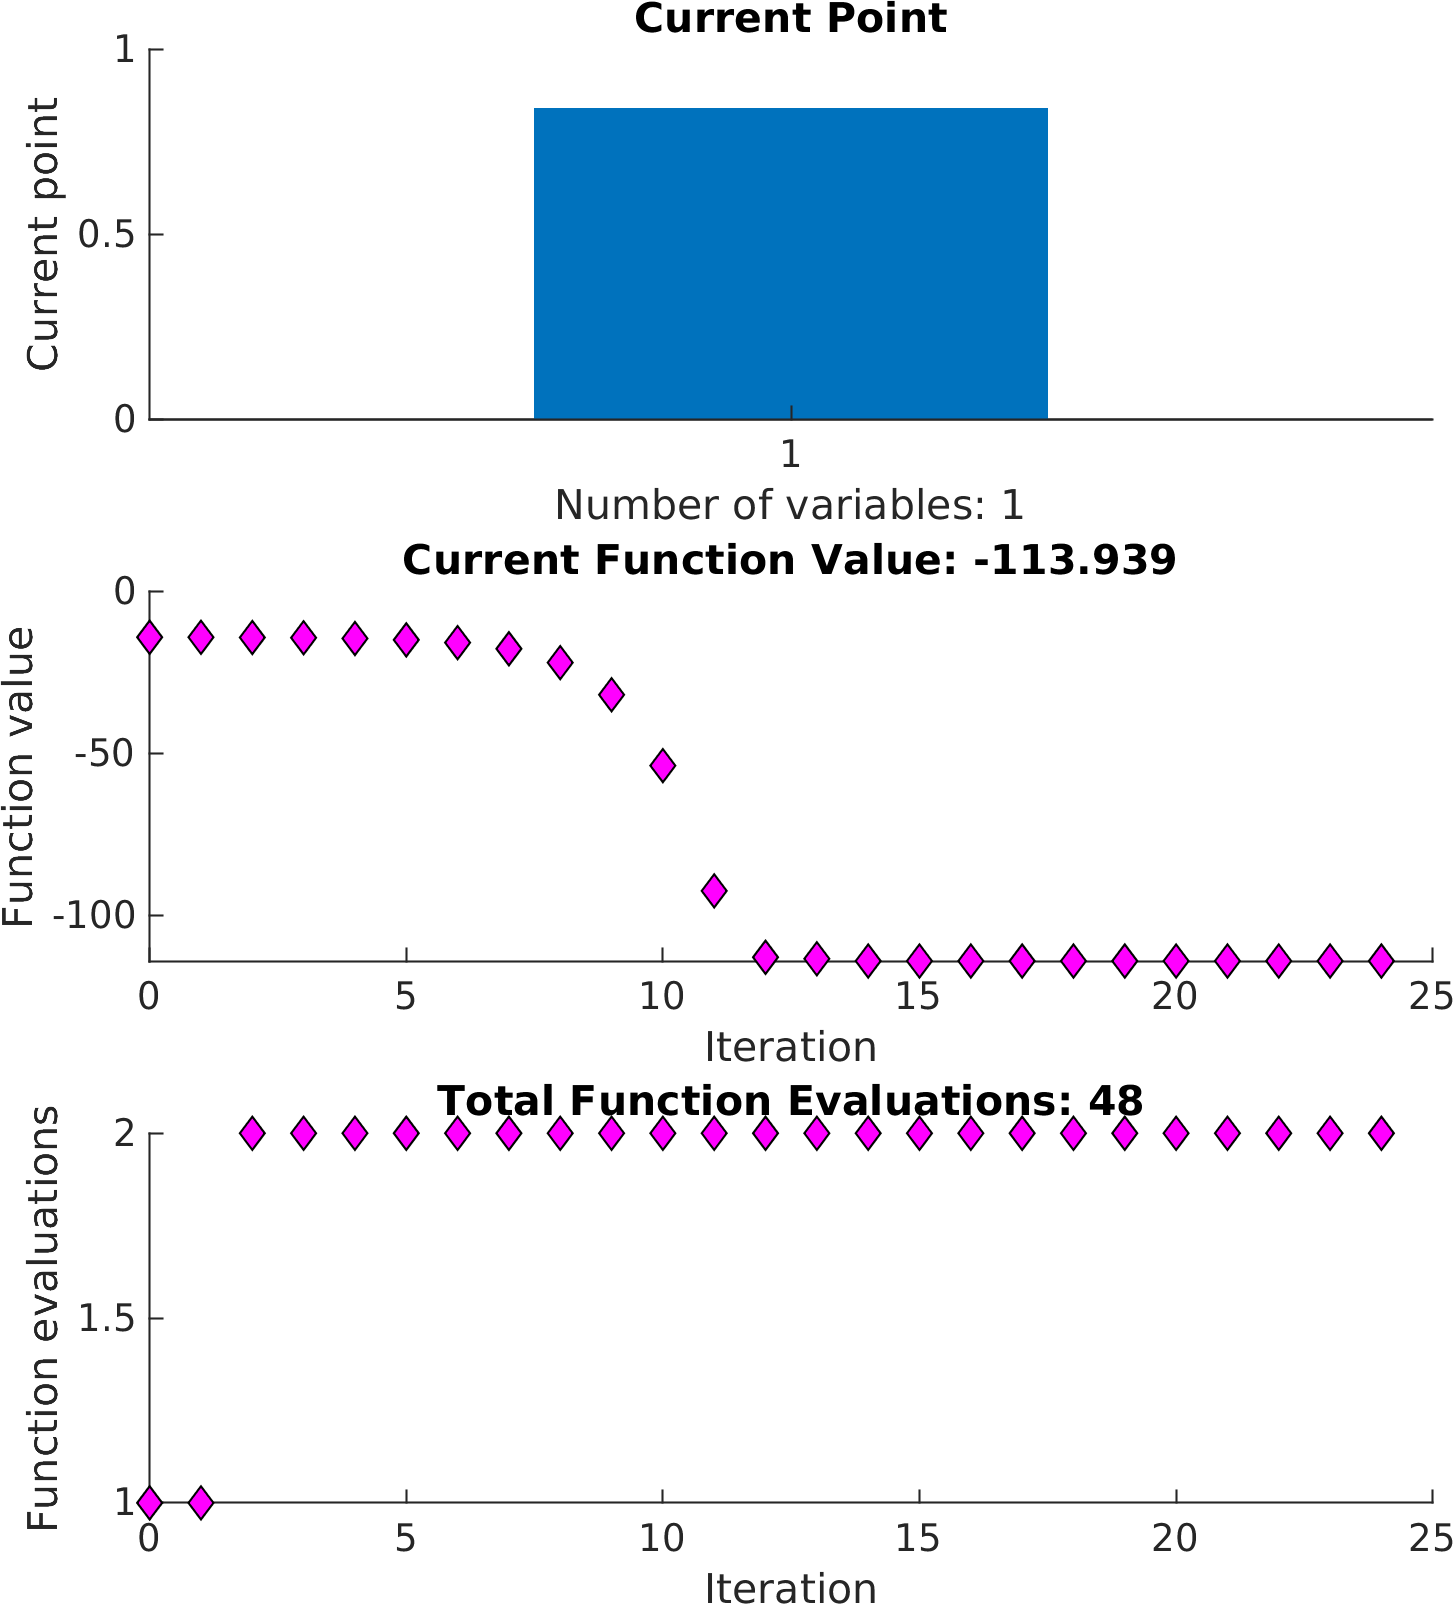
\includegraphics[width=0.6\textwidth]{../code/chap13/opt_plot.png}}
    \caption{Figure resulting from setting \\ \lstinline{'PlotFcns' = {@optimplotx, @optimplotfval, @optimplotfunccount}}}
    \label{f:opt_plot}
    \end{figure}

The two additional output variables also help us make sure the answer we received is what we intended.
\begin{code}
exitflag =
     1
output = 
  struct with fields:

    iterations: 24
     funcCount: 48
     algorithm: 'Nelder-Mead simplex direct search'
       message: 'Optimization terminated: the current x satisfies the 
       termination criteria using OPTIONS.TolX of 1.000000e-04 
        and F(X) satisfies the convergence criteria using 
        OPTIONS.TolFun of 1.000000e-04 '
\end{code}
The \lstinline{exitflag} will be \lstinline{1} when the solution converged, \lstinline{0} when it exceeds the allowed number of iterations and \lstinline{-1} if the search ended do to a user-defined exit criteria---similar to the event function we used with \lstinline{ode45}.   The \lstinline{output} variable is a structure with fields to characterize the process.

\clearpage

\section{Animation}

Animation is a useful tool for checking the results of a physical model. If something is wrong, animation can make it obvious. There are two ways to do animation in MATLAB. One is to use \lstinline{getframe} to capture a series of images and then use \lstinline{movie} to play them back.  This method is a bit involved, but allows you to generate a standalone video file, for example, a MP4 file.

\index{animation}
\index{getframe@\lstinline{getframe}}

The more informal way is to draw a series of plots.  You may have seen this when MATLAB incrementally generated the plots in Figure~\ref{f:opt_plot}  Listing~\ref{lst:animate} is a snippet that animates the results of a baseball simulation:

\begin{lstlisting}[caption={A snippet that animates the results of a baseball simulation}, label={lst:animate}]
    % Animate
    % Solve with ode45
    tspan = [0 10];
    xx_init = [0 30 1 40];
    options = odeset('Events', @event_landing);
    [tout, Xout] = ode45(@state_transition, tspan, xx_init, options);
    
    % Setup figure
    figure(4);
    clf();
    x = Xout(:,1);
    y = Xout(:,3);
    minmax = [min([x]), max([x]), min([y]), max([y])];
    % Plot each element in the solution
    for ii=1:round(length(tout)*4/5)
        clf; 
        hold on;
        plot(x(1:ii), y(1:ii), 'b:')
        plot(x(ii), y(ii), 'ro')
        axis(minmax)
        xlabel('x position [m]')
        ylabel('y position [m]')
        drawnow;
        if ii < length(tout)
            dt = tout(ii+1) - tout(ii);
            pause(dt);
        end
    end
\end{lstlisting}

A vector of four elements, \lstinline{minmax} is used inside the loop to set the axes of the figure.
This is necessary because otherwise MATLAB scales the figure each time through the loop,
so the axes keep changing, which makes the animation hard to watch.

\index{clf@\lstinline{clf}}
\index{clear figure}

Each time through the loop, \lstinline{animate} uses \lstinline{clf}
to clear the figure and \lstinline{axis} to reset the axes.  Then it plots a circle to represent the position of the \mbox{baseball}.

\index{drawnow@\lstinline{drawnow}}

We have to call \lstinline{drawnow} after \lstinline{plot} so
that MATLAB actually displays each plot.  Otherwise it waits
until you finish drawing all the figures and then updates
the display.

One limitation of this kind of animation is that the speed
of the animation depends on how fast your computer can generate
the plots.  Since the results from \lstinline{ode45} are usually not
equally spaced in time, your animation might slow down where
\lstinline{ode45} takes small time steps and speed up where the time
steps are larger.

\index{ode45@\lstinline{ode45}}
\index{time span}

One way to fix this problem is to change the way we specify \lstinline{tspan}.
Here's an example:

\begin{code}
    tspan = 0:0.1:10;
\end{code}

The result is a vector that goes from 0 to 10 with a step size of 0.1.
Passing \lstinline{tspan} to \lstinline{ode45} in this form doesn't affect the accuracy of the results;
\lstinline{ode45} still uses variable time steps to generate the estimates, but then it interpolates them before returning the results.

\index{step size}
\index{pause@\lstinline{pause}}

With equal time steps, the animation should be smoother.

Another option is to use \lstinline{pause} to play the animation in
real time.  After drawing each frame and calling
\lstinline{drawnow}, you can compute the time
until the next frame and use \lstinline{pause} to wait:

\begin{code}
    dt = tout(ii+1) - tout(ii);
    pause(dt);
\end{code}

A limitation of this method is that it ignores the time required to
draw the figure, so it tends to run slow, especially if the figure is
complex or the time step is small.

\section{Chapter Review}

This chapter presented two new tools, \lstinline{fminsearch} and \lstinline{animate}.
The MATLAB function \lstinline{fminsearch} searches efficiently for the minimum of a function and can be adapted to search for the maximum, too.
The \lstinline{animate} function is one I wrote to read results from \lstinline{ode45} and generate an animation; the version in this chapter works with the results from the baseball simulation, but it can be adapted for other simulations.

In the exercises below, you have a chance to extend the example from this chapter and bring together many of the tools we have used so far.

In the next chapter, we move on to a new example, celestial mechanics, which describes the motion of planets and other bodies in outer space.


\section{Exercises}

Before you go on, you might want to work on the following exercises.

\begin{ex}

\index{Manny Ramirez}
\index{Boston Red Sox}

Manny Ramirez is a former member of the Boston Red Sox who was famous for his relaxed attitude.  The goal of this exercise is to solve the following Manny-inspired problem:

\begin{quote}
What is the minimum effort required to hit a home run in Fenway~Park?
\end{quote}

\index{Fenway Park}

Fenway Park is a baseball stadium in Boston, Massachusetts.  One of its most famous features is the ``Green Monster,'' which is a wall in left field that is unusually close to home plate, only 310 feet away.  To compensate for the short distance, the wall is unusually high, at 37 feet.

\index{Ramirez, Manny}
\index{Fenway Park}
\index{baseball}
\index{Green Monster}
\index{velocity}

You can solve this problem in two steps:

\begin{enumerate}

\item For a given velocity, find the launch angle that maximizes the height of the ball when it reaches the wall.  Notice that this is not quite the same as the angle that maximizes the distance the ball travels.

\index{launch angle}

\item Find the minimal velocity that clears the wall, given that it has the optimal launch angle.  Hint: this is actually a root-finding problem, not an optimization problem.

\end{enumerate}

\end{ex}


\begin{ex}
\label{golf}

\index{golf ball}
\index{force!Magnus}
\index{Magnus force}

A golf ball hit with backspin generates lift, which might increase the distance it travels, but the energy that goes into generating spin probably comes at the cost of lower initial velocity.

Write a simulation of the flight of a golf ball and use it to find
the launch angle and allocation of spin and initial velocity
(for a fixed energy budget) that maximizes the horizontal range of the
ball in the air.

The lift of a spinning ball is due to the Magnus force (see
\url{https://greenteapress.com/matlab/magnus}), which is
perpendicular to the axis of spin and the path of flight.  The
coefficient of lift is proportional to the spin rate; for a ball
spinning at 3000~rpm it is about 0.1.  The coefficient of drag of a
golf ball is about 0.2 as long as the ball is moving faster than \SI{20}{\meter\per\second}.

\end{ex}
